%This is a very basic  BE PROJECT PRELIMINARY template.

%############################################# 
%#########Author :  PROJECT###########
%#########COMPUTER ENGINEERING############


\documentclass[oneside,a4paper,12pt]{report}
\usepackage{graphicx}
\usepackage{amsmath}
\usepackage{fancyhdr}
\usepackage{titlesec}
%\usepackage{showframe}
%\hoffset = 8.9436619718309859154929577464789pt
%\voffset = 13.028169014084507042253521126761pt

\fancypagestyle{plain}{%
  \fancyhf{}
  \fancyfoot[CE]{College_Name, Department of Computer Engineering 2025-26}
  \fancyfoot[RE]{\thepage}
}
\pagestyle{fancy}
\fancyhead{}
\renewcommand{\headrulewidth}{0pt}
\footskip = 0.625in
\cfoot{}
\rfoot{}

\usepackage[]{hyperref}
\usepackage{tikz}
\usetikzlibrary{arrows,shapes,snakes,automata,backgrounds,petri,positioning,fit}

\usepackage{tabularx}
\usepackage{longtable}

\usepackage[nottoc,notlot,notlof,numbib]{tocbibind}
\usepackage[titletoc]{appendix}
\usepackage{titletoc}
\renewcommand{\appendixname}{Annexure}
\renewcommand{\bibname}{References}

\setcounter{secnumdepth}{5}

\usepackage{float}
\usepackage{subcaption}
\usepackage{multirow}

\usepackage[ruled,vlined]{algorithm2e}

\begin{document}

\setlength{\parindent}{0mm}
\begin{center}
{\bfseries SAVITRIBAI PHULE PUNE UNIVERSITY \\}
 \vspace*{1\baselineskip}

\includegraphics[width=100pt]{logo.png}
 \vspace*{0.5\baselineskip}
 
{\bfseries A FINAL PROJECT REPORT \\}
{\bfseries ON \\}
 \vspace*{1\baselineskip}
{\bfseries \fontsize{16}{12} \selectfont Image Geolocation and Hazard-Aware Response \\ \vspace*{2\baselineskip}}
{\fontsize{12}{12} \selectfont SUBMITTED TOWARDS THE
 \\PARTIAL FULFILLMENT OF THE REQUIREMENTS OF \\

\vspace*{1\baselineskip}}
{\bfseries \fontsize{14}{12} \selectfont BACHELOR OF ENGINEERING  \\
\vspace{1\baselineskip}} 
{\bfseries \fontsize{14}{12} \selectfont BY \\}

\begin{tabular}{l @{\hspace{25mm}} l}
Bhargav Dave & Exam No: B401220231 \\
Nibodh Daware & Exam No: B401220232  \\
Kiran Raut & Exam No: B401220347 \\
Shreyash Borge & Exam No: B401220216\\
\end{tabular}
\vspace*{1\baselineskip}\\
{\bfseries \fontsize{14}{12} \selectfont Under The Guidance of \\  
\vspace{1mm}} 
Mrs. Dipti S. Chaudhari\\
\vspace*{1\baselineskip} 

\includegraphics[width=100pt]{pccoer.jpg} \\
{\bfseries \fontsize{14}{12} \selectfont DEPARTMENT OF COMPUTER ENGINEERING \\
Pimpri Chinchwad College of Engineering And Research \\
Ravet \\
A.Y. 2025--2026
}
\end{center}

\newpage



\begin{figure}[ht]
\centering

\includegraphics[width=100pt]{pccoer.jpg}
\end{figure}

{\bfseries \fontsize{14}{12} \selectfont \centerline{Pimpri Chinchwad College Of Engineering And Research}
\centerline{DEPARTMENT OF COMPUTER ENGINEERING}
\vspace*{2\baselineskip}} 


{\bfseries \fontsize{16}{12} \selectfont \centerline{CERTIFICATE} 
\vspace{1\baselineskip}} 

\centerline{This is to certify that the Project Entitled}
\vspace*{1\baselineskip} 


{\bfseries \fontsize{14}{12} \selectfont \centerline{Image Geolocation and Hazard-Aware Response}
\vspace*{1\baselineskip}}

\centerline{Submitted by}
\begin{center}
\begin{tabular}{l @{\hspace{25mm}} l}
Bhargav Dave & Exam No: B401220231 \\
Nibodh Daware & Exam No: B401220232  \\
Kiran Raut & Exam No: B401220347 \\
Shreyash Borge & Exam No: B401220216\\
\end{tabular}
\end{center}
\vspace*{1\baselineskip} 
is a bonafide work carried out by Students under the supervision of {\bfseries Mrs. Dipti S. Chaudhari} and it is submitted towards the partial fulfillment of the requirement of {\bfseries Bachelor of Engineering} (Computer Engineering) Project.\\\\

\bgroup
\def\arraystretch{0.7}
\begin{tabular}{c c }
Mrs. Dipti S. Chaudhari &  \hspace{50 mm} Dr. Vijay Kotkar \\								
{\bfseries Internal Guide}   &  {\bfseries \hspace{50 mm} H.O.D} \\
{\bfseries Dept. of Computer Engg.}  &	{\bfseries \hspace{50 mm}Dept. of Computer Engg.}  \\
\\
\vspace*{8\baselineskip} 
\end{tabular}

\begin{tabular}{c c }
Dr. Shivganga V. Gavhane &  \hspace{50 mm} Prof.Dr. H.U.Tiwari \\		{\bfseries Project Co-ordinator}   &  {\bfseries \hspace{50 mm} Director} \\ 
\\\\

\vspace*{2\baselineskip} 
{\bfseries EXTERNAL SIGNATURE} & \hspace{60 mm} 
\end{tabular}
\egroup



%}



\newpage

%\pictcertificate{TITLE OF BE PROJECT}{Student Name}{Exam Seat No}{Guide Name}
\setcounter{page}{0}

\cfoot{Department of Computer Engineering, PCCOER Ravet, 2025-26}
\rfoot{\thepage}
\pagenumbering{Roman}
%\pictack{BE PROJECT TITLE}{Guide Name}

		
{  \newpage {\bfseries \fontsize{14}{12} \selectfont \centerline{Acknowledgments} 
\vspace*{2\baselineskip}} \setlength{\parindent}{11mm} }
{ \setlength{\parindent}{0mm} }

It gives us great pleasure in presenting the final project report on {\bfseries \fontsize{12}{12} \selectfont `Image Geolocation and Hazard-Aware Response'}.
\vspace*{1\baselineskip}

We take this opportunity to express our sincere gratitude to our internal guide \textbf{Prof. Mrs. Dipti S. Chaudhari} for her constant guidance, technical suggestions, and encouragement throughout the development of this project. Her feedback helped us refine the project scope, system architecture, safety constraints, and evaluation approach.
\vspace*{1\baselineskip}

We are thankful to \textbf{Prof. Shivganga V. Gavhane}, Project Co-ordinator, for her support during project reviews and documentation. We also express our gratitude to \textbf{Dr. Vijay Kotkar}, Head of Department, Department of Computer Engineering, PCCOER, Ravet, for providing the required academic support and infrastructure.
\vspace*{1\baselineskip}

We are heartily thankful to \textbf{Prof. Dr. H. U. Tiwari}, Director, PCCOER, Ravet, for providing a supportive research environment, laboratory facilities, and motivation to complete the project successfully.
\vspace*{1\baselineskip}

We also thank all teaching and non-teaching staff members, our classmates, and our families for their cooperation and encouragement during the completion of this work.
\vspace*{3\baselineskip} \\
\begin{tabular}{p{8.2cm}c}
Bhargav Dave\\
Nibodh Daware\\
Kiran Raut\\
Shreyash Borge\\
(B.E. Computer Engg.)
\end{tabular}

{  \newpage {\bfseries \fontsize{14}{12} \selectfont \centerline{Abstract} 
\vspace*{2\baselineskip}} \setlength{\parindent}{11mm} 
{ \setlength{\parindent}{0mm} } }

Image Geolocation and Hazard-Aware Response is a multimodal image understanding system that combines place-aware visual reasoning with risk-aware decision support. The system accepts an image from the user, analyzes visual and contextual cues using a vision-capable multimodal large language model, and returns a structured response containing summary, possible location, risk level, confidence, entities, rationale, and recommended actions. For normal landmark or place images, the system provides informational actions such as learn-more and map lookup. For hazardous or suspicious scenes, the system shows report-oriented safety actions only after explicit user confirmation.

The project is implemented as a Python Flask backend, SQLite persistence layer, and React-based web interface. Gemini 2.5 Flash is used as the primary multimodal model, while deterministic post-processing logic validates model output, normalizes confidence, applies hazard keyword rules, and maps risk states to user-facing actions. The system stores sessions, messages, model outputs, actions, and incident records for auditability. The evaluation uses project run logs containing 22 analyzed runs across 14 sessions. Low-risk and high-risk outputs each occurred eight times, uncertain outputs occurred six times, and the average confidence was 0.623. Ten user-confirmed incident records and twelve learn-more actions were logged. The results show that structured multimodal reasoning can support both geospatial understanding and controlled hazard response, while preserving human verification for safety-sensitive actions.



% \maketitle
\tableofcontents
\listoffigures 
\listoftables



\clearpage
\pagenumbering{arabic}



  \titleformat{\chapter}[display]
{\thispagestyle{empty}\vspace*{\fill}\centering\bfseries}
{\huge CHAPTER \thechapter}
{0pt}
{\huge\uppercase}
[\vspace*{\fill}\newpage]







\setlength{\parindent}{11mm}
\chapter{Introduction}

\section{Overview}
The project titled \textbf{Image Geolocation and Hazard-Aware Response} is a chat-style multimodal system for image understanding, place identification, risk triage, and guided user action. The system allows a user to upload an image and receive an interpretable analysis of the scene. The response includes a short summary, possible location, detected entities, risk level, confidence score, explanation, and action buttons.

The project is developed as a web application. The frontend is implemented using React, Vite, TypeScript, Tailwind CSS, and reusable UI components. The backend is implemented using Python Flask with Pydantic validation and SQLite persistence. The primary model provider is Gemini Vision, configured to return strict JSON output. The system converts this structured model output into deterministic user actions such as \textit{Learn More}, \textit{Open Map}, \textit{Safety Tips}, \textit{Why this result?}, and \textit{Report Suspicious Activity}.

\section{Need and Relevance}
Images are widely shared during travel, public events, accidents, disasters, and suspicious activities. A normal image may require contextual information about a place, while a risky image may require safe reporting guidance. Traditional image geolocation systems mainly focus on predicting a place, but practical users also need risk-aware interpretation and accountable action support.

The proposed system is relevant because it joins image understanding with controlled decision support. It does not automatically notify authorities. Instead, it provides a human-in-the-loop flow where reporting is performed only after explicit user confirmation. This makes the system suitable for academic demonstration, public safety awareness, and image-based information retrieval.

\section{Motivation}
The motivation behind the project is to move beyond simple image classification or geolocation and build a usable multimodal assistant. Existing visual models can identify landmarks and describe scenes, but their responses are often free-form and difficult to audit. In safety-related scenarios, unsupported or overconfident claims can be harmful.

Therefore, the project uses structured output, validation, deterministic policy rules, and local logging. This makes the system behavior easier to explain during evaluation and safer for demonstrations involving possible hazards.

\section{Problem Statement}
To design and implement a multimodal web-based system that analyzes user-uploaded images, identifies possible location and scene context, detects hazard signals, and provides risk-aware actions with auditable user-confirmed reporting.

\section{Aim and Objectives}
The aim of the project is to develop an interpretable multimodal image analysis system that combines geospatial reasoning with hazard-aware decision support.

{\bfseries Objectives:}
\begin{itemize}
\item To develop a chat-style web interface for uploading and previewing images.
\item To integrate a vision-capable multimodal model for structured image analysis.
\item To validate and normalize model outputs into summary, risk level, confidence, entities, location, and rationale.
\item To implement deterministic risk-to-action mapping for normal, uncertain, medium-risk, and high-risk scenes.
\item To provide learn-more, map, safety, explanation, and user-confirmed report actions.
\item To persist sessions, messages, model outputs, actions, and incidents for audit and evaluation.
\item To evaluate the system using project test images and stored run logs.
\end{itemize}

\section{Project Scope and Limitations}
The project scope includes image upload, multimodal inference, structured response validation, confidence normalization, hazard-aware action mapping, learn-more lookup, optional map links, incident logging, and optional environment-gated WhatsApp notification after explicit confirmation.

The project does not include automatic emergency dispatch, legal identity verification, production-grade authentication, large-scale geotagged image retrieval, or forensic-level hazard verification. The current evaluation is based on a small project dataset and local run logs, so statistical conclusions are limited.

\section{Organisation of the Report}
Chapter 1 introduces the project, motivation, problem statement, objectives, scope, and limitations. Chapter 2 presents the literature survey and research gap analysis. Chapter 3 describes the software requirement specification, use cases, data model, and functional model. Chapter 4 presents the project plan, estimates, risk management, and team organization. Chapter 5 explains system design, architecture, mathematical model, data design, and results. Chapter 6 presents advantages, limitations, and applications. Chapter 7 describes validation and testing. Chapter 8 concludes the report and presents future scope.


\chapter{Literature Survey}

\section{Overview of Existing Research}
Image geolocation and visual place recognition have been studied using retrieval-based methods, deep convolutional networks, and recent vision-language models. Early systems used local visual descriptors and large geotagged image collections for nearest-neighbor matching \cite{lowe2004distinctive,vo2017revisiting}. Later approaches converted geolocation into classification over geographic regions or retrieval over learned place embeddings \cite{weyand2016planet,arandjelovic2016netvlad}. Recent multimodal foundation models combine image understanding with natural language reasoning, allowing richer scene interpretation and more flexible user interaction \cite{radford2021clip,li2023blip2,liu2024llava,team2024gemini}.

Hazard-aware visual decision support is related to explainable artificial intelligence, structured model outputs, safety policy design, and audit logging. In practical systems, location prediction alone is not enough. The system must also indicate uncertainty, provide rationale, and avoid automatic escalation without human confirmation. Retrieval-grounded and reasoning-based geolocation studies motivate stronger evidence linking, but most existing work still focuses on benchmark geolocation instead of incident-response workflow \cite{zhou2024img2loc,li2025pixels,yerramilli2025geochain}.

\section{Literature Survey}
\begingroup
\scriptsize
\renewcommand{\arraystretch}{1.18}
\setlength{\tabcolsep}{3pt}
\begin{longtable}{|p{0.055\textwidth}|p{0.22\textwidth}|p{0.12\textwidth}|p{0.18\textwidth}|p{0.19\textwidth}|p{0.19\textwidth}|}
\caption{Literature Survey}
\label{tab:litsurvey}\\
\hline
\textbf{Sr. No} & \textbf{Paper Title} & \textbf{Journal / Conference} & \textbf{Authors \& Year} & \textbf{Methodology} & \textbf{Research Gap} \\
\hline
\endfirsthead
\hline
\textbf{Sr. No} & \textbf{Paper Title} & \textbf{Journal / Conference} & \textbf{Authors \& Year} & \textbf{Methodology} & \textbf{Research Gap} \\
\hline
\endhead
1 & PlaNet - Photo Geolocation with Convolutional Neural Networks & ECCV & Weyand, Kostrikov and Philbin, 2016 & CNN-based geolocation classification over geographic cells. & Strong geolocation focus, but limited explainability and no hazard-aware actions. \\
\hline
2 & Revisiting IM2GPS in the Deep Learning Era & ICCV & Vo, Jacobs and Hays, 2017 & Retrieval and deep feature based geolocation. & Depends on visual similarity datasets and does not provide decision-support workflow. \\
\hline
3 & Learning Transferable Visual Models From Natural Language Supervision & ICML & Radford et al., 2021 & Contrastive image-text pretraining for transferable visual representation. & Powerful visual-language alignment, but not directly designed for safety escalation. \\
\hline
4 & PIGEON: Predicting Image Geolocations & CVPR & Haas, Skreta, Alberti and Finn, 2024 & Multimodal geolocation using foundation model reasoning. & Geolocation performance is emphasized more than operational user actions. \\
\hline
5 & Img2Loc: Revisiting Image Geolocalization using Multi-modality Foundation Models and Image-based Retrieval-Augmented Generation & SIGIR & Zhou et al., 2024 & Foundation model plus retrieval-augmented image geolocation. & Retrieval grounding is useful, but incident logging and hazard response are outside scope. \\
\hline
6 & LLMGeo: Benchmarking Large Language Models on Image Geolocation In-the-wild & arXiv & Wang et al., 2024 & Benchmarking multimodal language models for geolocation. & Benchmarks model ability, but does not implement a complete safety-aware application. \\
\hline
7 & Improving Image Geolocation with Multimodal Deep Learning & ICONIP & Sinski, Zychowski and Mandziuk, 2024 & Uses multimodal deep learning for image geolocation improvement. & Focuses on geolocation improvement, not user-confirmed hazard reporting. \\
\hline
8 & IM2City: Image Geo-localization via Multi-modal Learning & ACM SIGSPATIAL Workshop & Wu and Huang, 2022 & Combines image and auxiliary modality cues for city-scale localization. & City-level localization does not directly support safety triage actions. \\
\hline
9 & Tell Me Where You Are: Multimodal LLMs Meet Place Recognition & arXiv & Lyu et al., 2024 & Evaluates multimodal LLMs for place recognition and contextual location reasoning. & Does not include incident persistence or notification policy. \\
\hline
10 & BLIP-2: Bootstrapping Language-Image Pre-training with Frozen Image Encoders and Large Language Models & ICML & Li et al., 2023 & Aligns frozen image encoders with large language models using lightweight querying. & General vision-language method without domain-specific hazard action mapping. \\
\hline
11 & VLM-Guided Visual Place Recognition for Planet-Scale Geo-Localization & arXiv & Waheed et al., 2025 & Uses VLM guidance for large-scale visual place recognition. & Emphasizes retrieval quality, not controlled user-facing report workflow. \\
\hline
12 & From Pixels to Places: A Systematic Benchmark for Evaluating Image Geolocation Ability in Large Language Models & arXiv & Li et al., 2025 & Benchmarks LLM geolocation ability across image-to-place tasks. & Evaluation is benchmark-oriented and does not measure incident action outcomes. \\
\hline
13 & GeoChain: Multimodal Chain-of-Thought for Geographic Reasoning & EMNLP Findings & Yerramilli et al., 2025 & Decomposes geographic reasoning using multimodal chain-of-thought. & Reasoning improves explainability, but operational safety logging is outside scope. \\
\hline
14 & GeoGuess: Multimodal Reasoning based on Hierarchy of Visual Information in Street View & arXiv & Cheng et al., 2025 & Uses hierarchical visual information for street-view geolocation reasoning. & Street-view reasoning is not directly integrated with emergency response actions. \\
\hline
15 & Distinctive Image Features from Scale-Invariant Keypoints & IJCV & Lowe, 2004 & Introduces SIFT local features for robust image matching. & Classical matching lacks semantic risk understanding and natural language rationale. \\
\hline
16 & Visual Place Recognition with Repetitive Structures & IEEE TPAMI & Torii et al., 2015 & Improves place recognition under repeated urban structures and viewpoint changes. & Robust place matching does not classify hazard severity or confidence-based action paths. \\
\hline
17 & NetVLAD: CNN Architecture for Weakly Supervised Place Recognition & CVPR & Arandjelovic et al., 2016 & Learns compact place descriptors using weak supervision. & Retrieval descriptors alone do not provide explainable safety decisions. \\
\hline
18 & SuperGlue: Learning Feature Matching with Graph Neural Networks & CVPR & Sarlin et al., 2020 & Learns graph-based feature matching for reliable correspondences. & Useful for visual evidence but not a complete multimodal decision-support system. \\
\hline
19 & Visual Instruction Tuning & NeurIPS & Liu et al., 2024 & Trains instruction-following vision-language assistants. & General assistant behavior still requires project-specific validation and policy control. \\
\hline
20 & Gemini: A Family of Highly Capable Multimodal Models & arXiv & Gemini Team, 2024 & Describes a family of multimodal models for text, image, and reasoning tasks. & Model capability alone does not define auditable incident workflow or local system policy. \\
\hline
\end{longtable}
\endgroup

\section{Research Gap Analysis}
The reviewed literature shows significant progress in image geolocation, visual place recognition, and vision-language reasoning. However, most approaches are evaluated using location accuracy, retrieval performance, or benchmark scores. In real-world use, a user may need both place information and risk-aware guidance.

The main gaps identified are:
\begin{itemize}
\item Lack of combined geolocation and hazard-aware response in a single user-facing workflow.
\item Limited use of structured output validation for model responses.
\item Limited focus on deterministic action mapping from risk level and confidence.
\item Lack of human-confirmed incident reporting and audit logging in geolocation prototypes.
\item Limited confidence calibration and conservative fallback design for ambiguous images.
\end{itemize}

The proposed project addresses these gaps by combining multimodal image analysis, structured JSON output, deterministic policy rules, action buttons, and persistent logs for evaluation.


\chapter{Software Requirement Specification}

\section{Introduction}
\subsection{Purpose and Scope of Document}
Facilitating other Documentation: This SRS serves as a foundational reference for all future project documentation, including system design documents, test plans, user manuals, and project reports. It ensures consistency across development phases by providing a clear understanding of system requirements and expected behavior.

Product Validation: The SRS enables validation by establishing measurable criteria for evaluating the system's performance and verifying that the final implementation meets user requirements. It acts as a benchmark for acceptance testing to ensure the predicted geolocation results are accurate, reliable, and aligned with project objectives.

\subsection{Characteristics of a Software Requirement Specification}
Accuracy: The SRS clearly defines the functional and non-functional requirements without ambiguity. Every requirement accurately reflects the intended system behavior, such as input image handling, machine learning-based geolocation prediction, and result interpretation. Accurate details ensure developers and stakeholders share a common understanding.

Completeness: The SRS provides a complete description of all required system features, constraints, performance expectations, and interfaces. It includes functional requirements such as dataset processing, model training, and location prediction, as well as non-functional aspects like performance, security, usability, and scalability. No essential requirement is omitted.

Prioritization of Requirements: The requirements in the SRS are organized based on importance and implementation priority. Critical functionalities such as image preprocessing and model prediction are placed at higher priority, followed by enhancements like user interface improvements, accuracy tuning, and dataset expansion. Prioritization ensures efficient planning and phased development.

\subsection{Overview of Responsibilities of Developer}
The development responsibilities include frontend design, backend API implementation, multimodal model integration, database schema design, validation logic, safety policy implementation, and testing. The developer must ensure that the system does not perform automatic authority dispatch and that all report actions are explicitly confirmed by the user.

\section{Usage Scenario}
The system is designed for users who want to understand an image, identify possible place context, or receive safety-aware guidance. A user opens the web application, uploads an image, and submits it for analysis. The backend sends the image and prompt to the multimodal model, validates the returned JSON, applies policy rules, saves logs, and returns a response with actions.

\subsection{User Profiles}
\begin{table}[H]
\centering
\caption{System Entities Description}
\label{tab:entities}
\def\arraystretch{1.5}
\begin{tabularx}{\textwidth}{|c|l|X|}
\hline
\textbf{Sr. No.} & \textbf{Actor} & \textbf{Description} \\ \hline
1 & General User & Uploads an image and receives scene explanation, location estimate, risk level, and actions. \\ \hline
2 & Public Safety Observer & Uses the report flow when a hazardous or suspicious image is detected and confirms incident logging. \\ \hline
3 & Reviewer / Evaluator & Reviews stored model outputs, actions, confidence values, and incident records for project evaluation. \\ \hline
4 & System Administrator & Configures API keys, database path, upload size, and optional WhatsApp notification settings. \\ \hline
\end{tabularx}
\end{table}

\subsection{Use Cases}
\begin{table}[H]
\centering
\caption{Use Cases}
\label{tab:usecases}
\def\arraystretch{1.4}
\begin{tabularx}{\textwidth}{|c|X|X|c|X|}
\hline
\textbf{Sr. No.} & \textbf{Use Case} & \textbf{Description} & \textbf{Actors} & \textbf{Assumption}\\ \hline
1 & Analyze Image & User uploads an image and receives a structured scene interpretation. & User & Image format is supported. \\ \hline
2 & Learn More & User selects learn-more action for a normal landmark or place. & User & Place/entity is detected. \\ \hline
3 & Open Map & User opens a map search for the detected location. & User & Location guess is available. \\ \hline
4 & View Explanation & User checks why a result was produced. & User & Rationale is returned or fallback rationale exists. \\ \hline
5 & Report Suspicious Activity & User confirms incident reporting for high-risk output. & User & Confirmation is required before logging. \\ \hline
6 & Review Logs & Evaluator checks sessions, actions, and incidents. & Reviewer & Database records are available. \\ \hline
\end{tabularx}
\end{table}

\subsection{Use Case View}
The use case view represents interaction between users and the multimodal assistant. The primary user uploads an image and receives analysis. Based on the response, the user may learn more, open a map, view rationale, or confirm a report. The reviewer interacts with logs for evaluation.

\begin{figure}[H]
\centering
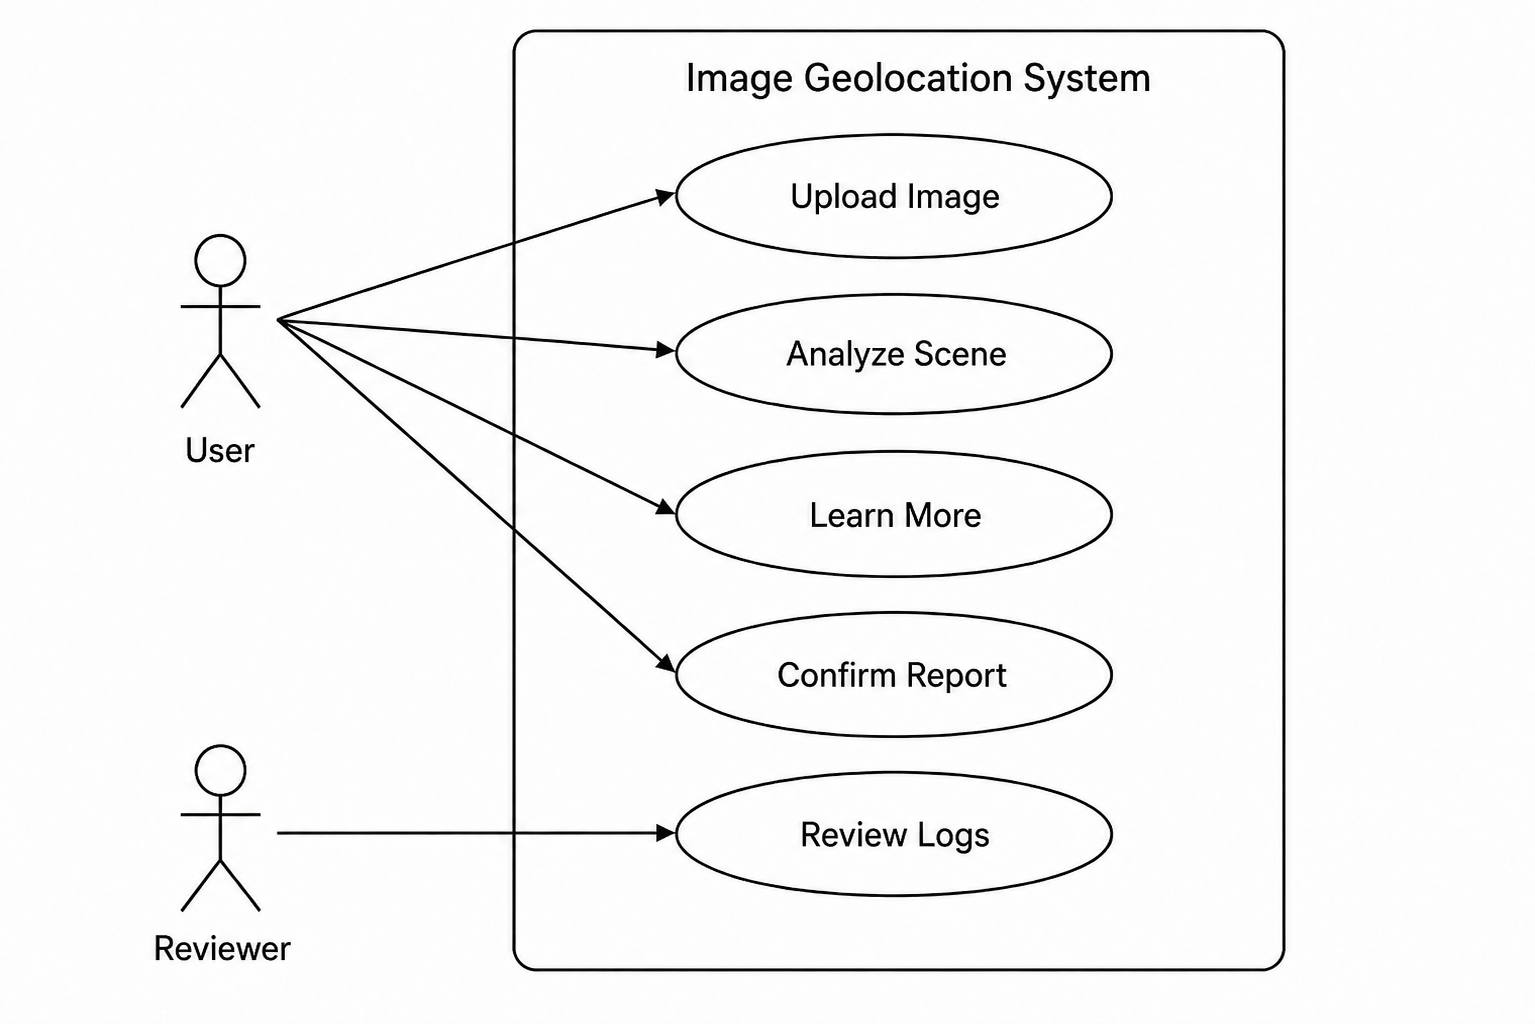
\includegraphics[width=0.95\textwidth]{diagrams/use-case.png}
\caption{Use case diagram}
\label{fig:usecase}
\end{figure}

\section{Data Model and Description}
\subsection{Data Description}
The system uses SQLite as the persistence layer. It stores session data, messages, structured model outputs, user actions, and incident records. Raw images are not stored by default; an image hash is saved for traceability and privacy.

\subsection{Data Objects and Relationships}
The main database tables are:
\begin{itemize}
\item \textbf{sessions}: Stores conversation sessions.
\item \textbf{messages}: Stores user and assistant messages with optional image hash.
\item \textbf{model\_outputs}: Stores risk level, confidence, and full JSON payload.
\item \textbf{actions}: Stores user-selected actions such as learn-more and report.
\item \textbf{incidents}: Stores user-confirmed incident reports and optional notification status.
\end{itemize}

\begin{figure}[H]
\centering
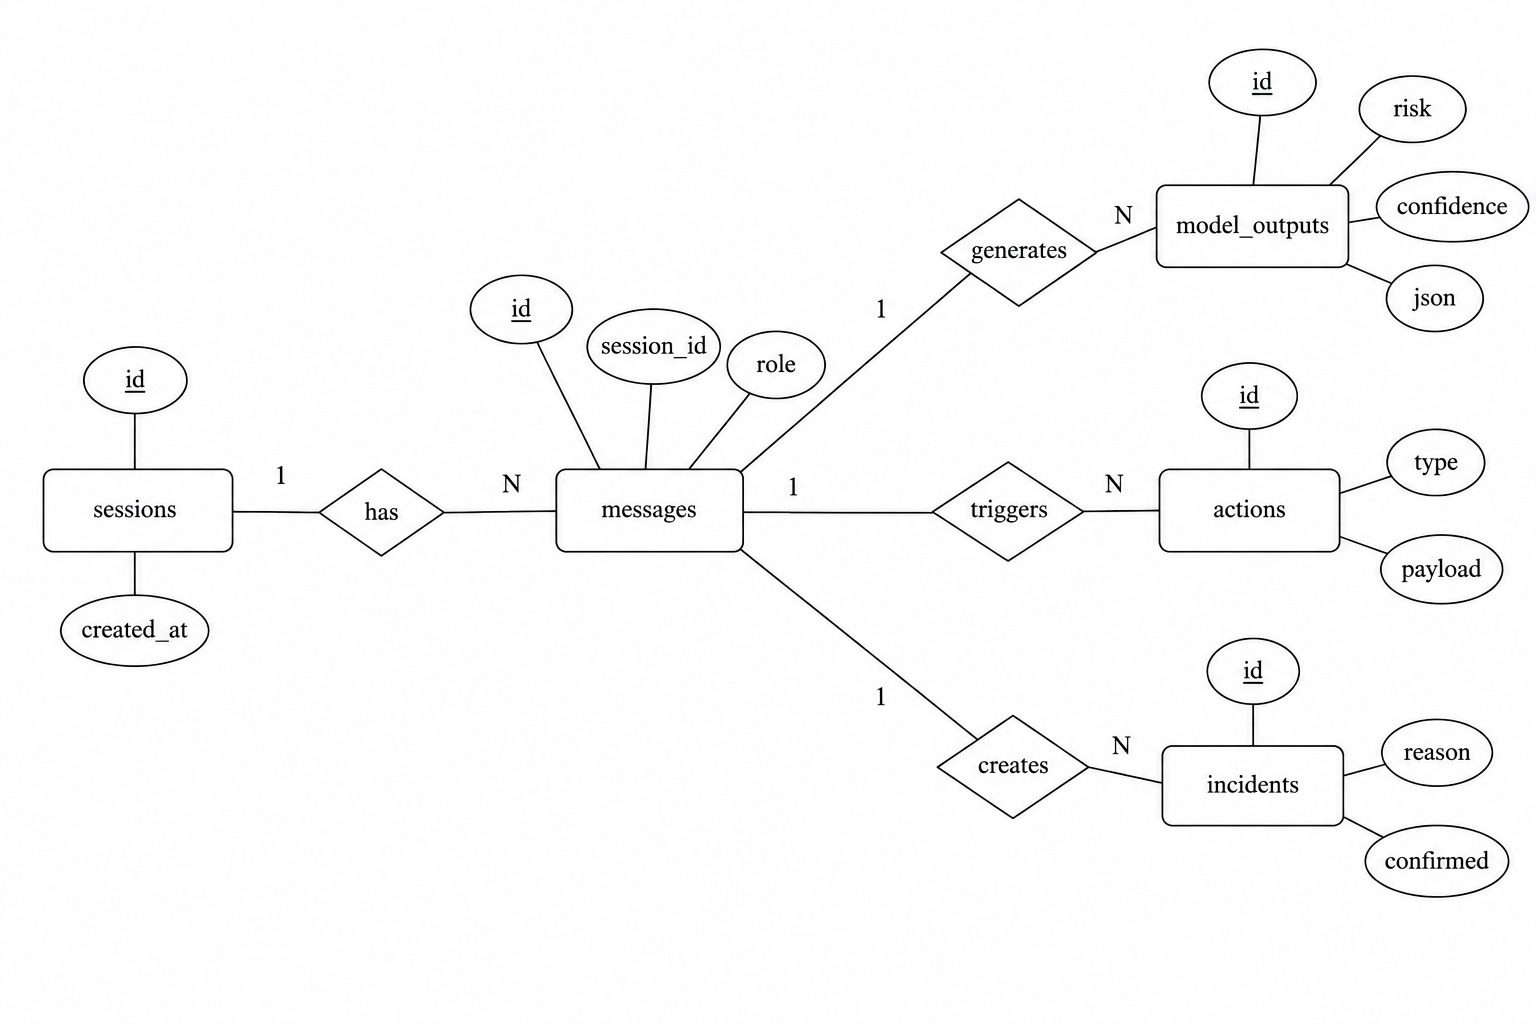
\includegraphics[width=0.95\textwidth]{diagrams/er-diagram.jpeg}
\caption{ER diagram}
\label{fig:er}
\end{figure}

\section{Functional Model and Description}
\subsection{Data Flow Diagram}
The data flow starts when a user submits an image. The frontend sends a multipart request to the backend. The backend validates input, hashes the image, invokes Gemini Vision, parses the model response, applies policy rules, saves records, and returns a response to the frontend.

\subsubsection{Level 0 Data Flow Diagram}
\begin{figure}[H]
\centering
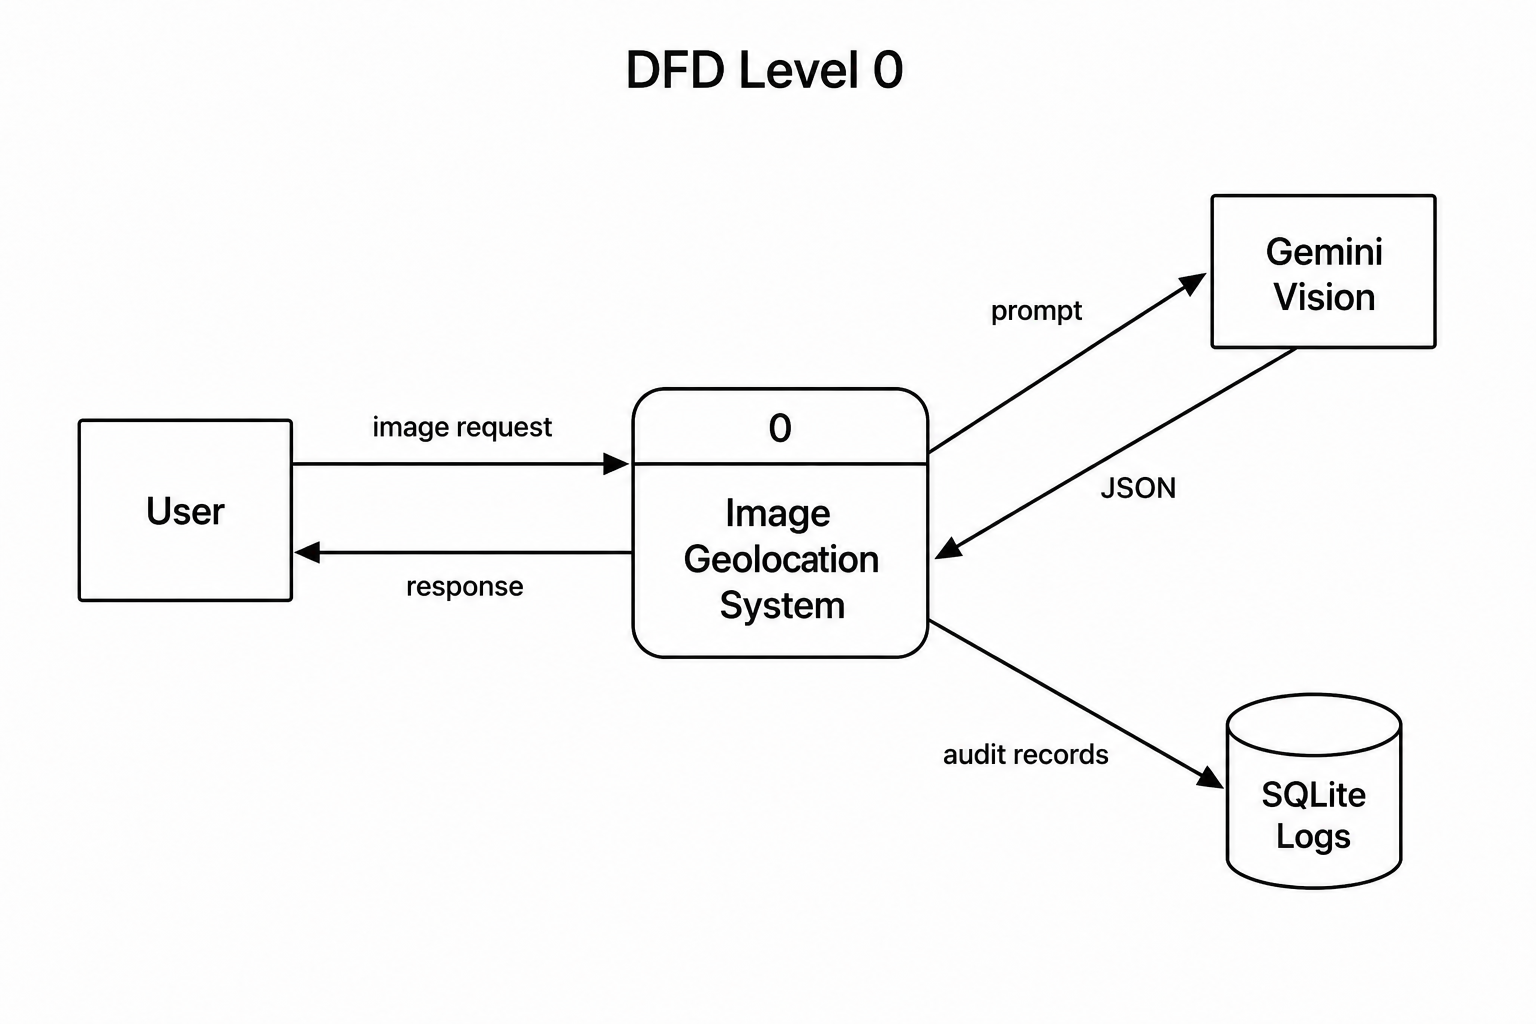
\includegraphics[width=0.95\textwidth]{diagrams/dfd-lvl-0.png}
\caption{DFD Level 0 diagram}
\label{fig:dfd0}
\end{figure}

\subsubsection{Level 1 Data Flow Diagram}
\begin{figure}[H]
\centering
\resizebox{0.92\textwidth}{!}{%
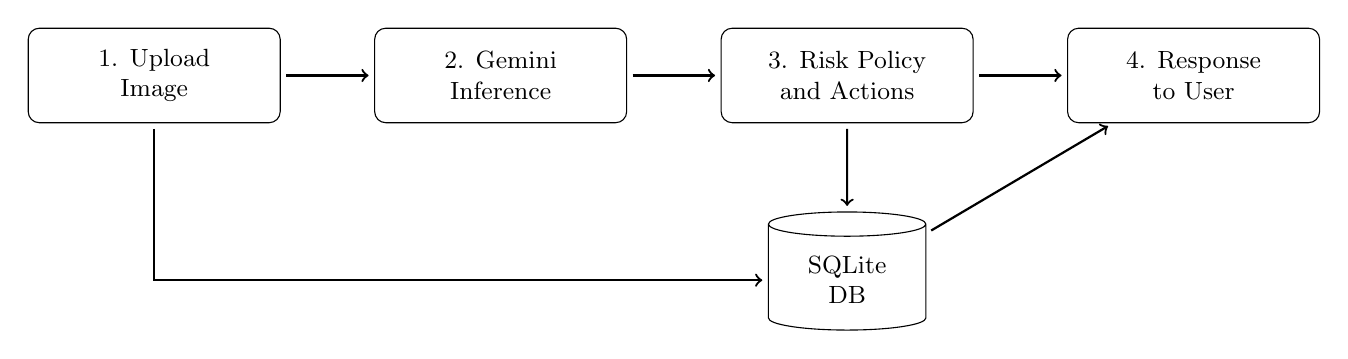
\begin{tikzpicture}[
process/.style={rectangle, draw, rounded corners, minimum width=32mm, minimum height=12mm, align=center, font=\small},
store/.style={cylinder, draw, shape border rotate=90, aspect=0.25, minimum height=15mm, minimum width=20mm, align=center, font=\small},
flow/.style={->, thick, shorten >=2pt, shorten <=2pt}
]
\node[process] (upload) at (0,0) {1. Upload\\Image};
\node[process] (infer) at (4.4,0) {2. Gemini\\Inference};
\node[process] (policy) at (8.8,0) {3. Risk Policy\\and Actions};
\node[process] (reply) at (13.2,0) {4. Response\\to User};
\node[store] (db) at (8.8,-2.6) {SQLite\\DB};
\draw[flow] (upload) -- (infer);
\draw[flow] (infer) -- (policy);
\draw[flow] (policy) -- (reply);
\draw[flow] (upload) |- (db);
\draw[flow] (policy) -- (db);
\draw[flow] (db) -- (reply);
\end{tikzpicture}
}
\caption{DFD Level 1 diagram}
\label{fig:dfd1}
\end{figure}

\subsection{Description of Functions}
The major functions of the system are image upload, model inference, JSON extraction, JSON repair, output normalization, hazard signal detection, action generation, learn-more lookup, map link generation, incident reporting, and audit logging.

\subsection{Activity Diagram}
The activity diagram represents the end-to-end workflow from image upload to action selection.

\begin{figure}[H]
\centering
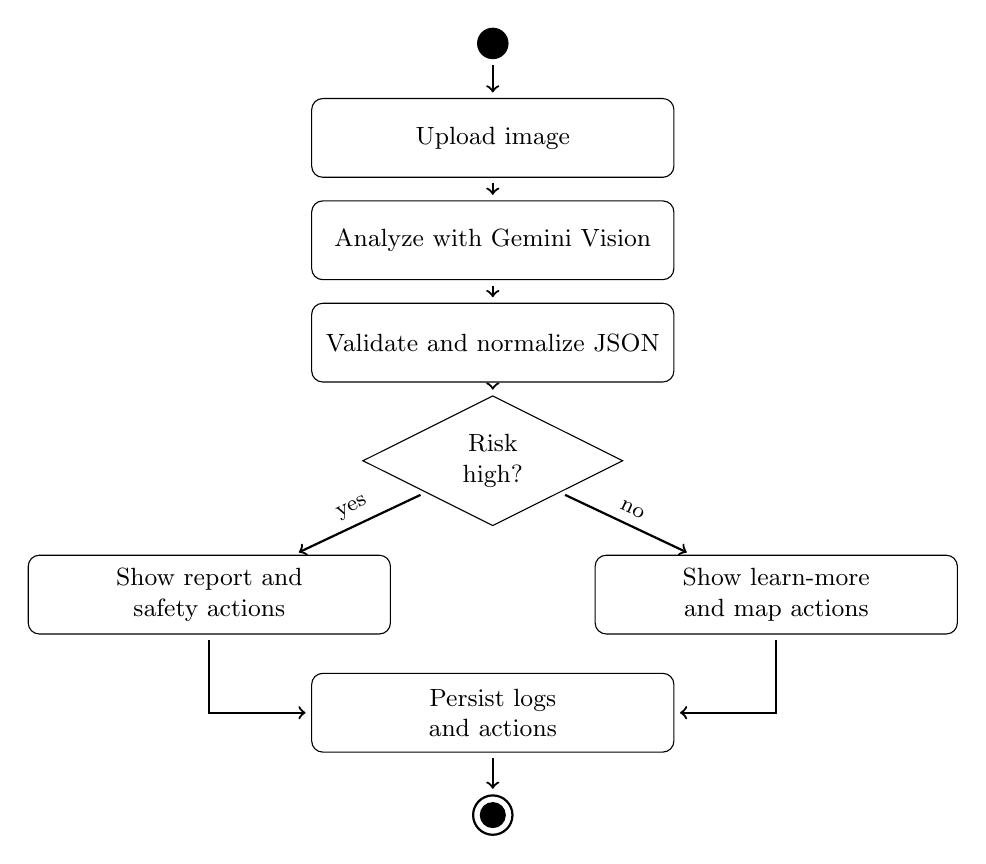
\begin{tikzpicture}[
activity/.style={rectangle, draw, rounded corners, minimum width=46mm, minimum height=10mm, align=center, font=\small},
decision/.style={diamond, draw, aspect=2, align=center, inner sep=2mm, font=\small},
flow/.style={->, thick, shorten >=2pt, shorten <=2pt}
]
\node[circle, fill=black, minimum size=4mm] (start) at (0,0) {};
\node[activity] (upload) at (0,-1.2) {Upload image};
\node[activity] (analyze) at (0,-2.5) {Analyze with Gemini Vision};
\node[activity] (normalize) at (0,-3.8) {Validate and normalize JSON};
\node[decision] (risk) at (0,-5.3) {Risk\\high?};
\node[activity] (report) at (-3.6,-7) {Show report and\\safety actions};
\node[activity] (learn) at (3.6,-7) {Show learn-more\\and map actions};
\node[activity] (persist) at (0,-8.5) {Persist logs\\and actions};
\node[circle, draw, thick, minimum size=5mm] (end) at (0,-9.8) {};
\node[circle, fill=black, minimum size=3mm] at (0,-9.8) {};
\draw[flow] (start) -- (upload);
\draw[flow] (upload) -- (analyze);
\draw[flow] (analyze) -- (normalize);
\draw[flow] (normalize) -- (risk);
\draw[flow] (risk) -- node[above, sloped, font=\footnotesize]{yes} (report);
\draw[flow] (risk) -- node[above, sloped, font=\footnotesize]{no} (learn);
\draw[flow] (report) |- (persist);
\draw[flow] (learn) |- (persist);
\draw[flow] (persist) -- (end);
\end{tikzpicture}
\caption{Activity diagram}
\label{fig:activity}
\end{figure}

\subsection{Non Functional Requirements}
\begin{itemize}
\item \textbf{Performance}: The MVP targets response latency below 8 seconds for common demo cases.
\item \textbf{Reliability}: Invalid model output must trigger repair or safe fallback.
\item \textbf{Security}: API keys must be stored in environment variables and not logged.
\item \textbf{Privacy}: Raw images are not stored by default; image hashes are persisted.
\item \textbf{Usability}: The interface must show image preview, chat messages, and inline action buttons.
\item \textbf{Auditability}: Every model output, action, and incident must be stored for review.
\end{itemize}

\subsection{State Diagram}
The system state changes from image selection to analysis, output generation, action rendering, and optional incident creation.

\begin{figure}[H]
\centering
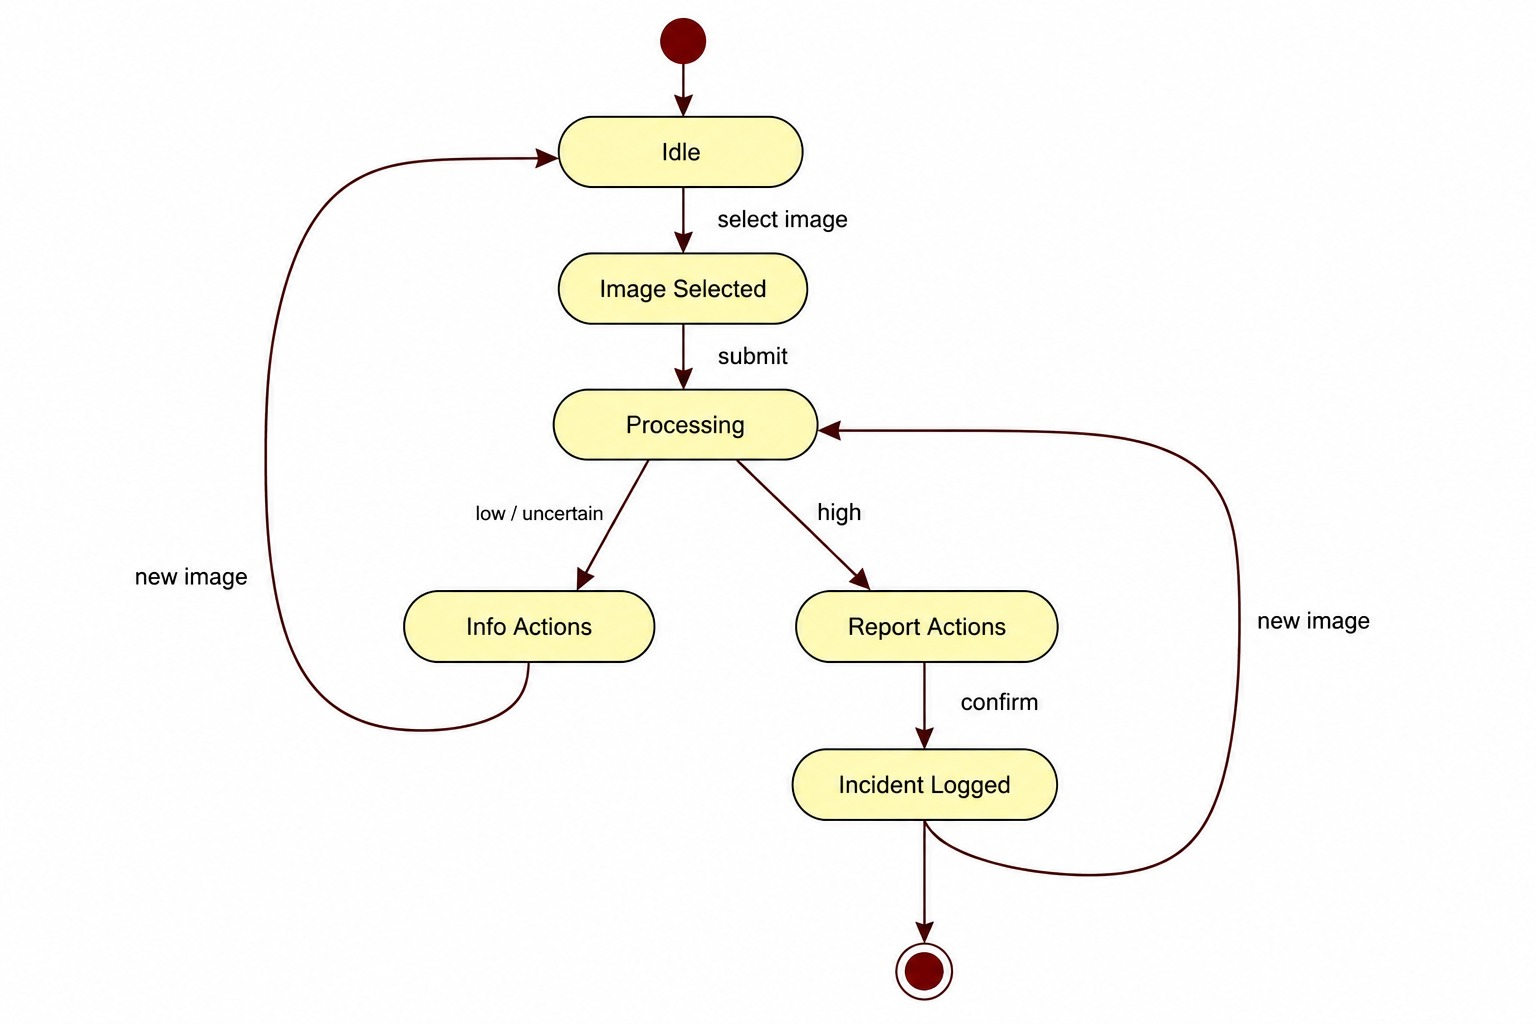
\includegraphics[width=0.95\textwidth]{diagrams/state-transition.jpeg}
\caption{State transition diagram}
\label{fig:state}
\end{figure}

\subsection{Design Constraints}
The system must not perform automatic external authority dispatch. WhatsApp notification is optional, environment-gated, and requires explicit user confirmation. The model must return strict JSON where possible, and fallback behavior must be conservative when confidence is low or output is invalid.

\subsection{Software Interface Description}
The backend exposes REST APIs for analysis, learn-more, report, and health check. The frontend communicates with these APIs using HTTP requests. Gemini Vision is accessed through the Google Generative Language API. Wikipedia is used for learn-more summaries, and Google Maps search links are generated for detected locations.


\chapter{Project Plan}

\section{Project Estimates}
The project was planned using an iterative software development approach. The work was divided into requirement analysis, literature survey, design, implementation, integration, testing, and documentation.

\begin{enumerate}
\item \textbf{Requirement Gathering}: The team studied the need for image geolocation, scene explanation, risk triage, user-confirmed reporting, and audit logging.
\item \textbf{Analysis}: Functional requirements, non-functional requirements, user roles, model constraints, and safety requirements were identified.
\item \textbf{Design}: The team designed the system architecture, data model, API flow, UI flow, and risk-to-action policy.
\item \textbf{Implementation}: The backend, frontend, database schema, model integration, action handlers, and incident logging were implemented.
\item \textbf{Testing}: Normal landmark images, hazardous images, ambiguous cases, learn-more actions, and report flows were tested.
\item \textbf{Documentation}: The final report, research paper, diagrams, results, limitations, and future scope were prepared.
\end{enumerate}

\subsection{Reconciled Estimates}
\subsubsection{Cost Estimate}
The project uses open-source development tools and academic infrastructure. The main cost components are internet usage, development machines, optional API usage, and documentation/printing. Since the prototype runs locally and uses SQLite, infrastructure cost is minimal.

\begin{table}[H]
\centering
\caption{Cost Estimate}
\begin{tabularx}{\textwidth}{|c|X|c|}
\hline
\textbf{Sr. No.} & \textbf{Resource} & \textbf{Estimated Cost} \\ \hline
1 & Development laptops and college laboratory facilities & Existing resources \\ \hline
2 & Open-source software tools & No direct cost \\ \hline
3 & Internet and API access for model testing & Variable / demo usage \\ \hline
4 & Report printing and binding & As per college requirement \\ \hline
\end{tabularx}
\end{table}

\subsubsection{Time Estimates}
\begin{table}[H]
\centering
\caption{Time Estimate}
\begin{tabularx}{\textwidth}{|c|X|c|}
\hline
\textbf{Sr. No.} & \textbf{Activity} & \textbf{Duration} \\ \hline
1 & Requirement analysis and literature survey & 3 weeks \\ \hline
2 & System design and database design & 2 weeks \\ \hline
3 & Backend and model integration & 4 weeks \\ \hline
4 & Frontend development and action workflow & 4 weeks \\ \hline
5 & Testing, metrics, and report preparation & 3 weeks \\ \hline
\end{tabularx}
\end{table}

\subsection{Project Resources}
\begin{itemize}
\item \textbf{People}: Four student developers, internal guide, project coordinator, and reviewers.
\item \textbf{Hardware}: Development laptops with internet connection.
\item \textbf{Software}: Python, Flask, SQLite, React, Vite, TypeScript, Tailwind CSS, Gemini Vision API, Wikipedia package, LaTeX.
\item \textbf{Tools}: VS Code, Git, browser developer tools, draw.io/diagram tools, pdflatex.
\end{itemize}

\section{Risk Management w.r.t. NP Hard Analysis}
The project is not an NP-hard optimization problem in the classical computational sense. However, it contains uncertainty and risk because visual scene interpretation, geolocation, and hazard detection are open-ended AI tasks. Risk management therefore focuses on model uncertainty, fallback behavior, API failure, privacy, and false alerts.

\subsection{Risk Identification}
\begin{itemize}
\item Model returns invalid or incomplete JSON.
\item Model produces incorrect location or risk level.
\item Hazard keyword fallback creates false alerts.
\item API key or network failure prevents model inference.
\item User reports an incident without proper context.
\item Raw image storage may create privacy concerns.
\end{itemize}

\subsection{Risk Analysis}
\begin{table}[H]
\begin{center}
\caption{Risk Table}
\label{tab:risk}
\def\arraystretch{1.4}
\begin{tabularx}{\textwidth}{|c|X|c|c|c|c|}
\hline
\multirow{2}{*}{ID} & \multirow{2}{*}{Risk Description} & \multirow{2}{*}{Probability} & \multicolumn{3}{|c|}{Impact} \\ \cline{4-6}
 & & & Schedule & Quality & Overall \\ \hline
1 & Invalid model output or parsing failure & Medium & Low & High & High \\ \hline
2 & Incorrect risk classification & Medium & Low & High & High \\ \hline
3 & Gemini API unavailable or key missing & Low & Medium & Medium & Medium \\ \hline
4 & False incident report by user & Low & Low & High & High \\ \hline
5 & Privacy concern due to image handling & Low & Low & High & High \\ \hline
\end{tabularx}
\end{center}
\end{table}

\subsection{Overview of Risk Mitigation, Monitoring, Management}
\begin{table}[H]
\centering
\caption{Risk Mitigation Plan}
\def\arraystretch{1.4}
\begin{tabularx}{\textwidth}{|c|X|X|}
\hline
\textbf{Risk ID} & \textbf{Mitigation Strategy} & \textbf{Monitoring Method} \\ \hline
1 & JSON extraction, one repair pass, and safe fallback response & Check model output logs \\ \hline
2 & Deterministic confidence thresholds and hazard policy rules & Review risk distribution and sample outputs \\ \hline
3 & Clear backend error handling and fallback messages & Monitor API response errors \\ \hline
4 & Require explicit user confirmation before incident creation & Review incident table \\ \hline
5 & Store image hash instead of raw image by default & Inspect message records and configuration \\ \hline
\end{tabularx}
\end{table}

\section{Project Schedule}
\subsection{Project Task Set}
\begin{itemize}
\item Task 1: Domain finalization and literature survey.
\item Task 2: Requirement analysis and SRS preparation.
\item Task 3: UI, API, database, and policy design.
\item Task 4: Backend implementation and Gemini integration.
\item Task 5: Frontend implementation and action buttons.
\item Task 6: Testing with normal, hazardous, and ambiguous images.
\item Task 7: Metrics analysis, report writing, and paper preparation.
\end{itemize}

\subsection{Task Network}
The task network follows a dependency chain: literature survey and requirements lead to architecture design; architecture design leads to backend and frontend implementation; implementation leads to testing; testing leads to result analysis and documentation.

\subsection{Timeline Chart}
\begin{table}[H]
\centering
\caption{Timeline Chart}
\def\arraystretch{1.3}
\begin{tabularx}{\textwidth}{|c|X|l|l|}
\hline
\textbf{Sr. No.} & \textbf{Task Name} & \textbf{Start Month} & \textbf{End Month} \\ \hline
1 & Domain study and base paper selection & June 2025 & July 2025 \\ \hline
2 & Requirement analysis and synopsis & August 2025 & September 2025 \\ \hline
3 & System design and diagrams & September 2025 & October 2025 \\ \hline
4 & Backend and database implementation & November 2025 & January 2026 \\ \hline
5 & Frontend and action workflow implementation & January 2026 & February 2026 \\ \hline
6 & Testing, evaluation, and report preparation & February 2026 & April 2026 \\ \hline
7 & Final documentation and submission & April 2026 & May 2026 \\ \hline
\end{tabularx}
\end{table}

\section{Team Organization}
\subsection{Team Structure}
The team consists of four student members working under the guidance of the internal guide. Responsibilities were distributed across research, backend, frontend, database, testing, documentation, and presentation.

\begin{figure}[H]
\centering
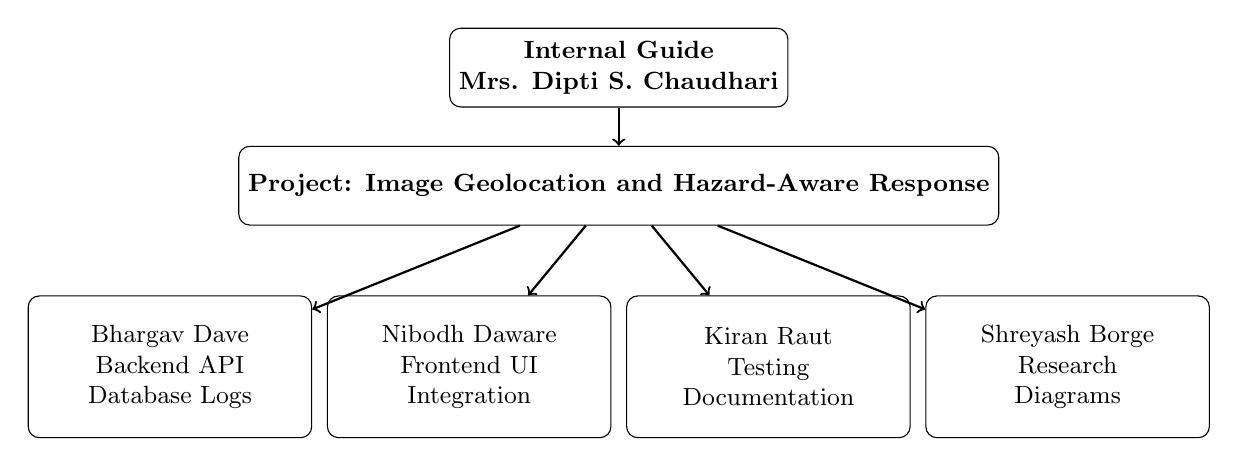
\begin{tikzpicture}[
member/.style={rectangle, draw, rounded corners, minimum width=36mm, minimum height=18mm, align=center, font=\small},
lead/.style={rectangle, draw, rounded corners, minimum width=42mm, minimum height=10mm, align=center, font=\small\bfseries},
flow/.style={->, thick}
]
\node[lead] (guide) at (5.7,1.8) {Internal Guide\\Mrs. Dipti S. Chaudhari};
\node[lead] (project) at (5.7,0.3) {Project: Image Geolocation and Hazard-Aware Response};
\node[member] (bhargav) at (0,-2.0) {Bhargav Dave\\Backend API\\Database Logs};
\node[member] (nibodh) at (3.8,-2.0) {Nibodh Daware\\Frontend UI\\Integration};
\node[member] (kiran) at (7.6,-2.0) {Kiran Raut\\Testing\\Documentation};
\node[member] (shreyash) at (11.4,-2.0) {Shreyash Borge\\Research\\Diagrams};
\draw[flow] (guide) -- (project);
\draw[flow] (project) -- (bhargav);
\draw[flow] (project) -- (nibodh);
\draw[flow] (project) -- (kiran);
\draw[flow] (project) -- (shreyash);
\end{tikzpicture}
\caption{Team structure}
\label{fig:team}
\end{figure}

\subsection{Management Reporting and Communication}
The team followed regular internal discussions, guide reviews, project lab sessions, and milestone-based reporting. Progress was tracked through working demonstrations, report updates, and review feedback.

\begin{table}[H]
\centering
\caption{Management Plan}
\def\arraystretch{1.3}
\begin{tabularx}{\textwidth}{|c|l|X|}
\hline
\textbf{Sr. No.} & \textbf{Month} & \textbf{Description} \\ \hline
1 & June-July & Domain discussion, paper search, and problem finalization. \\ \hline
2 & August-September & Requirement analysis, synopsis, and preliminary design. \\ \hline
3 & October-November & Architecture, database design, and backend planning. \\ \hline
4 & December-February & Implementation of backend, frontend, and action workflow. \\ \hline
5 & March-April & Testing, evaluation, metrics, and report drafting. \\ \hline
6 & May & Final report completion and submission preparation. \\ \hline
\end{tabularx}
\end{table}


\chapter{System Design}

\section{Introduction}
System design converts the requirements into a working architecture. The proposed system is designed as a client-server web application with a React frontend, Flask backend, SQLite database, and Gemini Vision model integration. The architecture separates user interaction, model inference, policy logic, action handling, and persistence.

\section{System Architecture Design}
The system architecture is shown in Fig. \ref{fig:systemarchitecture}. The frontend accepts image input and displays chat messages. The backend receives the request, validates input, sends the image to Gemini Vision, parses the response, applies normalization and risk rules, saves records, and returns action buttons to the frontend.

\begin{figure}[H]
\centering
\fbox{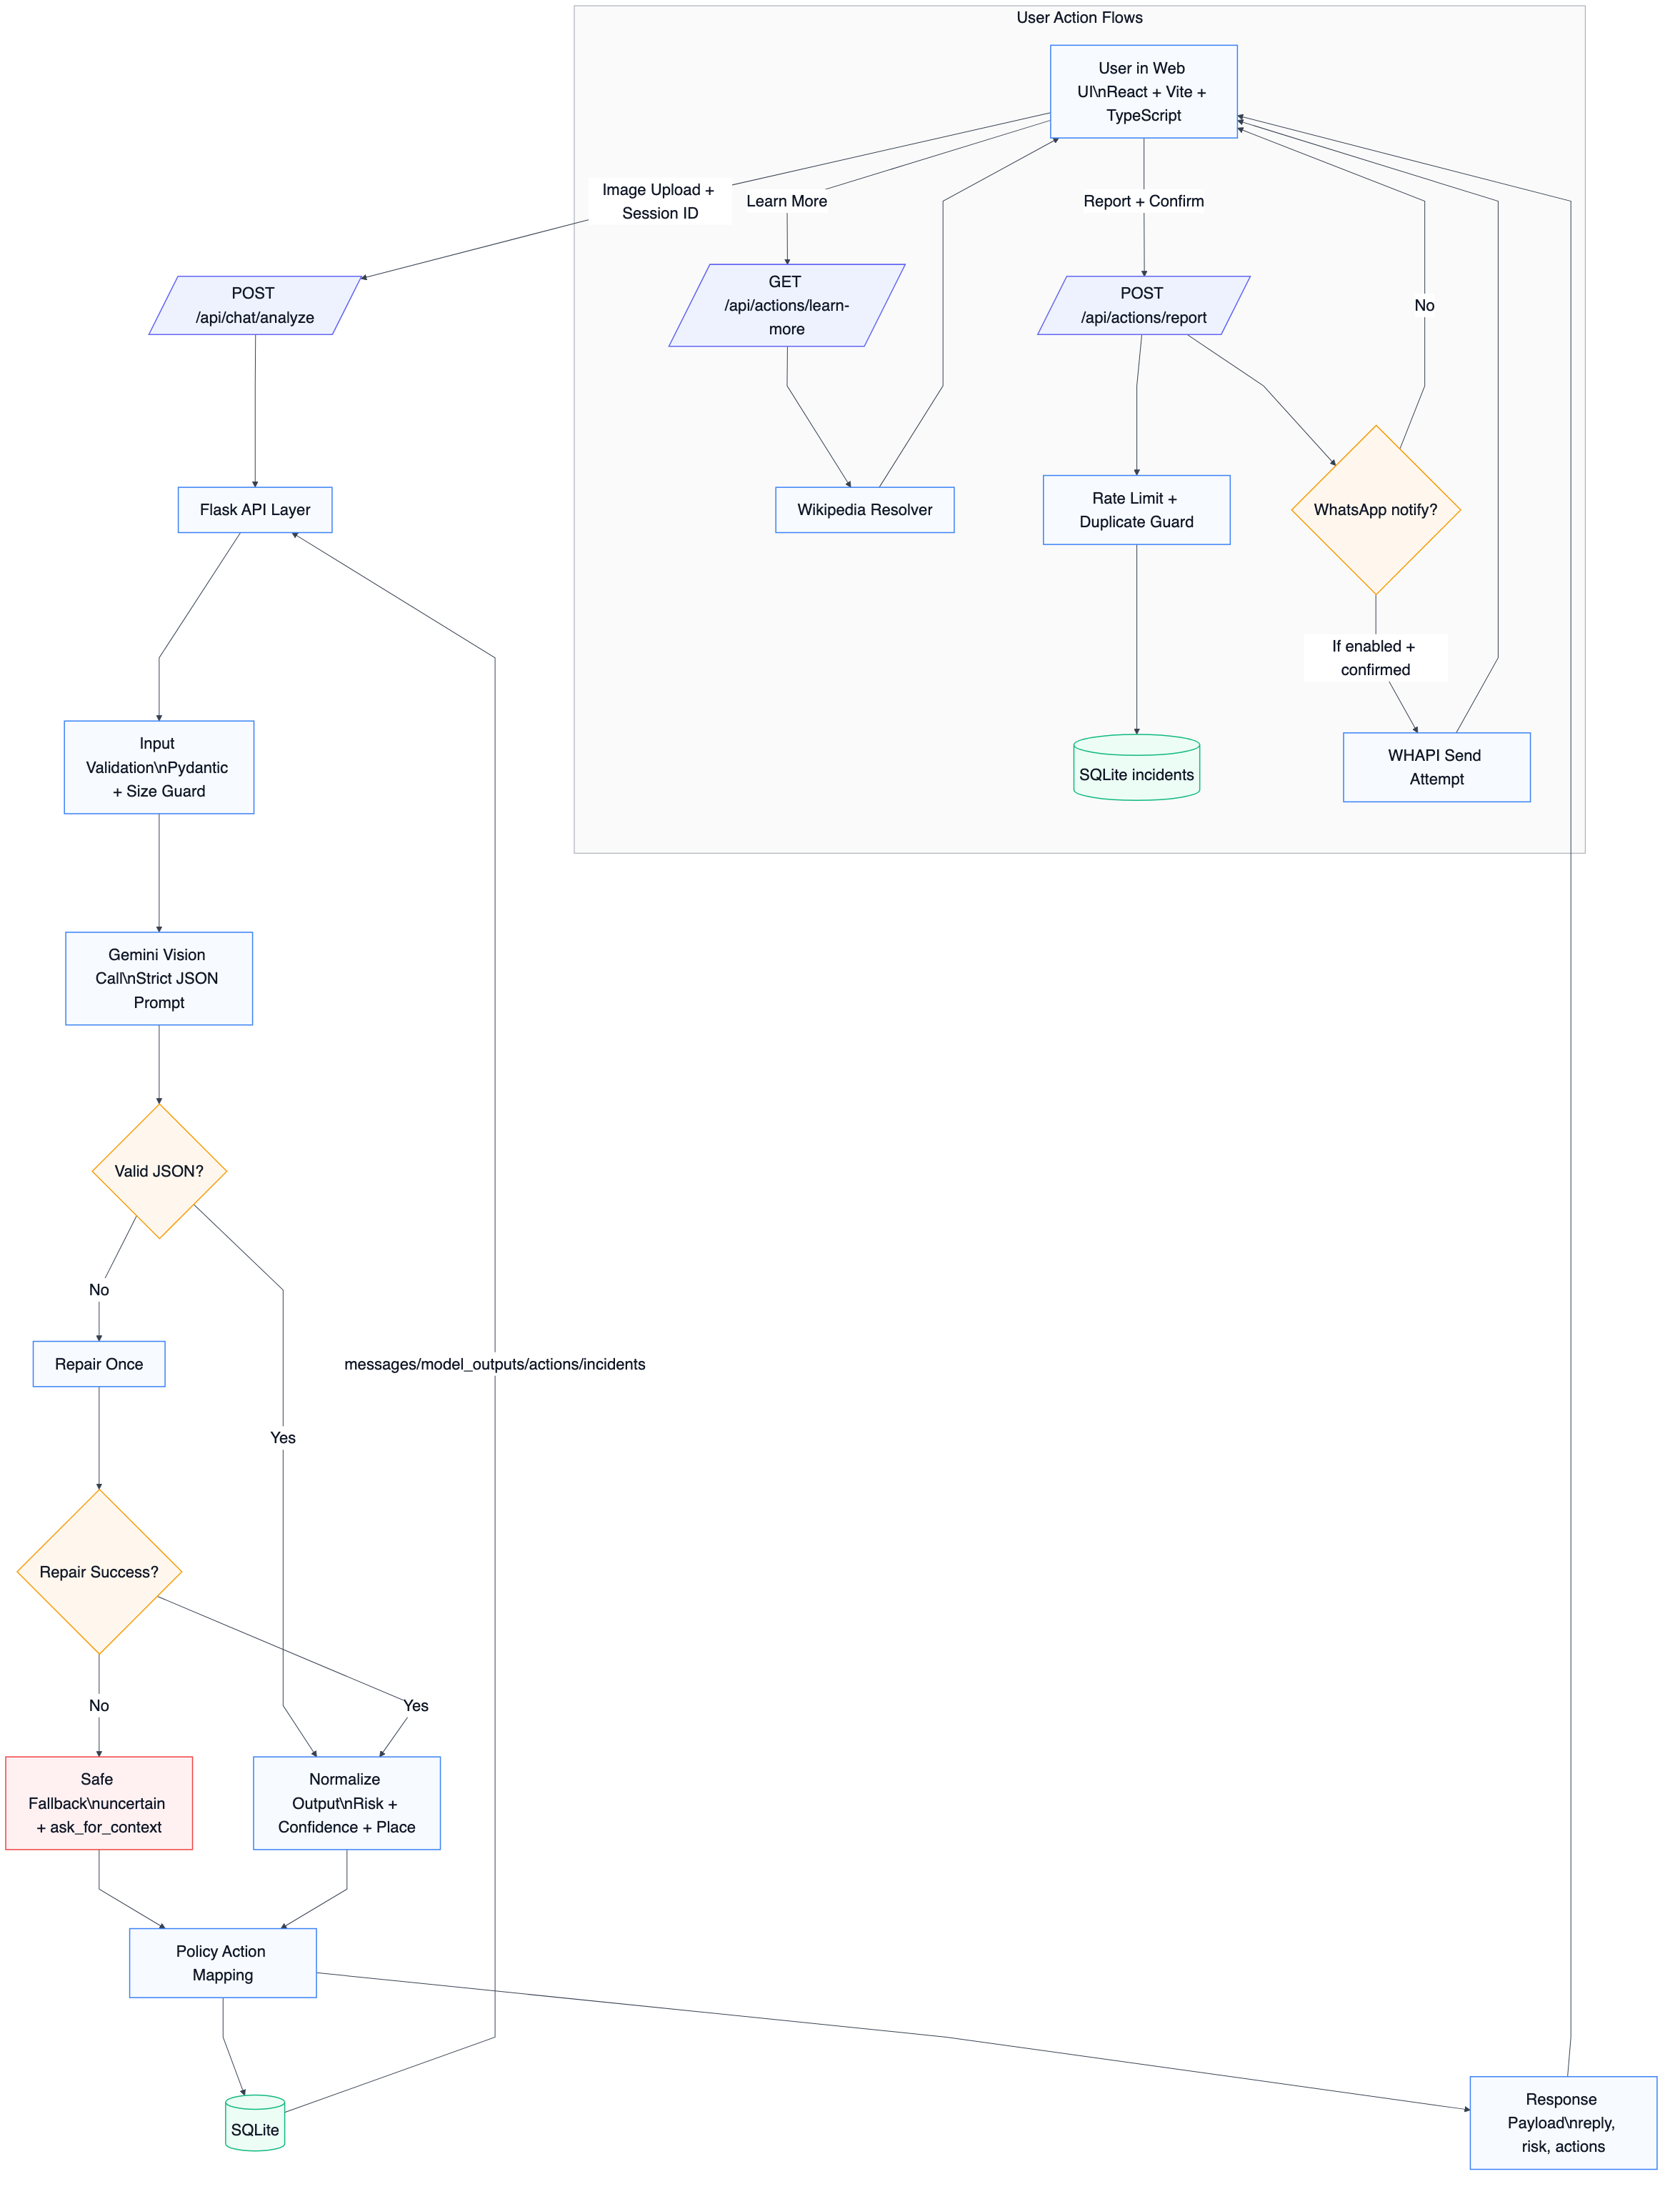
\includegraphics[width=0.95\textwidth]{../paper/figures/system_architecture.png}}
\caption{System architecture}
\label{fig:systemarchitecture}
\end{figure}

The main modules are:
\begin{itemize}
\item \textbf{User Interface}: Provides image upload, preview, chat timeline, and action buttons.
\item \textbf{Backend API}: Handles analyze, learn-more, report, and health endpoints.
\item \textbf{Multimodal Inference}: Sends image and prompt to Gemini Vision and requests strict JSON.
\item \textbf{Parser and Normalizer}: Extracts JSON, repairs invalid output once, validates fields, and normalizes confidence.
\item \textbf{Risk Policy}: Converts model output and hazard signals into final risk and confidence.
\item \textbf{Action Mapper}: Generates actions such as report, learn-more, open map, safety tips, and why.
\item \textbf{Persistence Layer}: Stores sessions, messages, model outputs, actions, and incidents in SQLite.
\end{itemize}

\section{Mathematical Model for the Proposed System}
Let the input image be represented by $I$ and optional user context be represented by $T$. The multimodal model produces a structured output:
\[
o = M(I,T)
\]
where $o$ contains summary, risk level, confidence, entities, possible location, rationale, and recommended actions.

Let $r_m$ be the model risk level and $c_m$ be the model confidence. Let $h=1$ if hazard keywords are present in the summary, rationale, user context, or location text; otherwise $h=0$. The final risk is:
\[
r =
\begin{cases}
\text{high}, & h=1 \text{ and } r_m \in \{\text{low, uncertain}\} \\
r_m, & \text{otherwise}
\end{cases}
\]

The confidence value is normalized to the range $[0,1]$. When a hazard signal is detected, the confidence is adjusted as:
\[
c = \max(c_m, 0.72) \quad \text{when } h=1
\]

The action set $A$ is selected using deterministic policy rules:
\[
A =
\begin{cases}
\{\text{ask\_for\_context}, \text{why}\}, & c < 0.45 \text{ or } r=\text{uncertain} \\
\{\text{report}, \text{safety\_tips}, \text{why}\}, & r=\text{high} \\
\{\text{safety\_tips}, \text{why}\}, & r=\text{medium} \\
\{\text{learn\_more}, \text{open\_map}, \text{why}\}, & r=\text{low}
\end{cases}
\]

\begin{algorithm}[H]
\caption{Hazard-Aware Image Analysis Flow}
\KwIn{Input image $I$ and optional message $T$}
\KwOut{Structured response and action set $A$}
Generate structured model output $o \leftarrow M(I,T)$\;
Extract JSON from model output\;
\If{JSON is invalid}{
Attempt one repair pass\;
}
\If{repair fails}{
Return safe fallback output\;
}
Normalize summary, risk, confidence, entities, and location\;
Detect hazard signal $h$\;
Apply risk and confidence policy\;
Generate action set $A$\;
Persist message, output, and action records\;
Return response to frontend\;
\end{algorithm}

\section{Data Design}
The internal data structure uses Python dictionaries and Pydantic models for API validation. The global data structure is the SQLite database. Temporary data includes uploaded image bytes, base64 encoded image content, parsed model JSON, and generated action payloads.

\subsection{Database Description}
\begin{table}[H]
\centering
\caption{Database Tables}
\def\arraystretch{1.4}
\begin{tabularx}{\textwidth}{|c|X|X|}
\hline
\textbf{Sr. No.} & \textbf{Table} & \textbf{Purpose} \\ \hline
1 & sessions & Stores unique user sessions and creation time. \\ \hline
2 & messages & Stores user and assistant messages with image hash. \\ \hline
3 & model\_outputs & Stores risk level, confidence, JSON payload, and timestamp. \\ \hline
4 & actions & Stores user action type and payload. \\ \hline
5 & incidents & Stores confirmed reports and notification status. \\ \hline
\end{tabularx}
\end{table}

\subsection{Component Design}
\begin{table}[H]
\centering
\caption{Component Design}
\def\arraystretch{1.4}
\begin{tabularx}{\textwidth}{|c|X|X|}
\hline
\textbf{Sr. No.} & \textbf{Component} & \textbf{Responsibility} \\ \hline
1 & React UI & Image upload, preview, chat display, and action button rendering. \\ \hline
2 & Flask API & Request handling, validation, response construction, and database operations. \\ \hline
3 & Gemini Integration & Multimodal image analysis and structured output generation. \\ \hline
4 & Policy Engine & Risk normalization, hazard keyword escalation, and action mapping. \\ \hline
5 & SQLite Store & Persistent audit logs for sessions, messages, outputs, actions, and incidents. \\ \hline
\end{tabularx}
\end{table}

\section{Results and Discussion}
The project evaluation uses available run logs. A run is one invocation of the image-analysis endpoint that produces one structured model output. The available evaluation set contains 22 runs across 14 sessions.

\begin{table}[H]
\centering
\caption{Available Dataset and Log Summary}
\begin{tabular}{|l|c|}
\hline
\textbf{Measure} & \textbf{Value} \\ \hline
Total analyzed runs & 22 \\ \hline
Distinct sessions & 14 \\ \hline
Low-risk outputs & 8 \\ \hline
High-risk outputs & 8 \\ \hline
Uncertain outputs & 6 \\ \hline
Average confidence & 0.623 \\ \hline
Confidence range & 0.00--0.95 \\ \hline
\end{tabular}
\end{table}

The reported confidence values are model confidence and policy-normalized confidence values, not independent expert accuracy labels. For the manually checked Shaniwar Wada case study, the system produced the expected action path for both samples: the regular image was classified as low risk with a learn-more action, and the fire-affected image was classified as high risk with a report action. Therefore, the verified case-study risk-action accuracy is 2 out of 2, or 100\%. A larger labelled test set is required to calculate precision, recall, and full hazard-classification accuracy.

\begin{table}[H]
\centering
\caption{Hazard-Action Outcome Summary}
\begin{tabular}{|l|c|}
\hline
\textbf{Outcome} & \textbf{Count} \\ \hline
User-confirmed incidents & 10 \\ \hline
Environment-enabled notification attempts & 3 \\ \hline
Successful notification sends & 3 \\ \hline
Local-only incident records & 7 \\ \hline
Report actions logged & 10 \\ \hline
Learn-more actions logged & 12 \\ \hline
\end{tabular}
\end{table}

Incident reporting and external notification are treated as separate stages. All ten incidents were user-confirmed and stored in SQLite. Only three of those reports had external notification enabled by the environment and user flow; all three enabled attempts were sent successfully.

\begin{figure}[H]
\centering
\begin{subfigure}{0.48\textwidth}
\centering

\includegraphics[height=5cm]{"../test/shaniwar_wada_cropped.jpg"}
\caption{Regular Shaniwar Wada image}
\end{subfigure}
\hfill
\begin{subfigure}{0.48\textwidth}
\centering

\includegraphics[height=5cm]{"../test/shaniwar_wada_flames_cropped.png"}
\caption{Hazardous Shaniwar Wada image}
\end{subfigure}
\caption{Test images used for case study}
\label{fig:shaniwar}
\end{figure}

For the normal Shaniwar Wada image, the stored output produced low risk with confidence 0.95 and the primary action was Learn More. For the fire-affected Shaniwar Wada image, the stored output produced high risk with confidence 0.85 and the primary action was Report. This demonstrates that the same place can receive different action paths depending on visual hazard evidence.


\chapter{Other Specifications}

\section{Advantages of the System}
\begin{itemize}
\item \textbf{Multimodal understanding}: The system can analyze image content along with user context.
\item \textbf{Structured output}: Model responses are converted into auditable fields instead of unstructured text only.
\item \textbf{Risk-aware actions}: The response changes based on risk level and confidence.
\item \textbf{Human-in-the-loop safety}: Incident reporting requires explicit confirmation from the user.
\item \textbf{Audit trail}: Sessions, messages, model outputs, actions, and incident records are persisted.
\item \textbf{Privacy-conscious storage}: Raw image storage is avoided by default and image hashes are stored.
\item \textbf{Extensible design}: The architecture can support additional models, retrieval systems, and notification providers in future.
\end{itemize}

\section{Limitations of the System}
\begin{itemize}
\item The evaluation dataset is small and limited to available project logs.
\item The system depends on the accuracy and availability of the multimodal model.
\item Hazard detection is not equivalent to legal or forensic verification.
\item Confidence scores are model-provided and require stronger calibration for production use.
\item The current implementation does not use vector database retrieval for geotagged image grounding.
\item Hazard demonstrations are mainly fire-related, while other emergency types need more testing.
\item The system does not include production-grade authentication, role-based access control, or legal compliance workflows.
\end{itemize}

\section{Applications of the System}
\begin{itemize}
\item Tourist landmark explanation and learn-more assistance.
\item Public safety awareness and guided incident reporting.
\item Academic demonstration of multimodal LLM-based decision support.
\item Image-based context retrieval for educational use.
\item Smart city monitoring support with human verification.
\item Disaster awareness prototypes for fire, flood, collapse, or other visible hazards.
\item Digital verification workflows where image context and explanation are required.
\end{itemize}


\chapter{Validation and Testing}

\section{Testing Methodology}
Testing was performed using functional testing, integration testing, UI testing, API testing, and log-based result validation. The focus was to verify that the system accepts images, returns structured responses, handles invalid model output safely, maps risk to correct actions, and persists records.

The testing flow was:
\begin{enumerate}
\item Upload normal landmark image.
\item Verify low-risk response and learn-more action.
\item Upload hazardous image.
\item Verify high-risk response and report action.
\item Test ambiguous or invalid response behavior.
\item Verify database records for messages, outputs, actions, and incidents.
\item Verify report confirmation and optional notification status.
\end{enumerate}

\section{Test Cases}
\begin{table}[H]
\centering
\caption{Test Case Summary}
\renewcommand{\arraystretch}{1.3}
\small
\begin{tabularx}{\textwidth}{|c|X|X|c|X|}
\hline
\textbf{Sr. No} & \textbf{Test Case Title / Description} & \textbf{Testing Methodology Applied} & \textbf{Result} & \textbf{Defects Identified} \\
\hline
1 & Upload supported image file and submit for analysis & Functional testing & PASS & None \\
\hline
2 & Analyze regular Shaniwar Wada image & System testing & PASS & None \\
\hline
3 & Analyze fire-affected Shaniwar Wada image & System testing & PASS & None \\
\hline
4 & Verify high-risk output shows Report action & Black-box testing & PASS & None \\
\hline
5 & Verify low-risk output shows Learn More and Open Map actions & Black-box testing & PASS & None \\
\hline
6 & Verify uncertain or low-confidence response asks for more context & Boundary testing & PASS & None \\
\hline
7 & Verify report action requires confirmation before incident creation & Functional testing & PASS & None \\
\hline
8 & Verify model output, action, and incident records are saved in SQLite & Integration testing & PASS & None \\
\hline
9 & Verify missing/invalid model response returns safe fallback & Negative testing & PASS & None \\
\hline
10 & Verify learn-more action fetches external knowledge summary & Integration testing & PASS & Depends on Wikipedia availability \\
\hline
\end{tabularx}
\end{table}

\section{Validation of Results}
The stored logs show 22 analyzed runs across 14 sessions. The risk distribution includes 8 low-risk outputs, 8 high-risk outputs, and 6 uncertain outputs. Confidence values range from 0.00 to 0.95 with an average of 0.623.

\begin{table}[H]
\centering
\caption{Confidence Band Distribution}
\begin{tabular}{|l|c|c|}
\hline
\textbf{Band} & \textbf{Count} & \textbf{Share} \\ \hline
Low ($<0.30$) & 6 & 27.3\% \\ \hline
Mid ($0.30$--$0.79$) & 5 & 22.7\% \\ \hline
High ($\geq0.80$) & 11 & 50.0\% \\ \hline
\end{tabular}
\end{table}

The case-study images validate the main intended behavior: the normal image leads to an informational action, while the hazardous image leads to a report-oriented action. The system therefore satisfies the MVP acceptance criteria for normal image interpretation, risky image escalation, ambiguity handling, and incident log review.


\chapter{Conclusion \& Future Scope}

\section{Conclusion}

This project successfully developed a multimodal image understanding system that integrates image geolocation, risk assessment, and guided action support. The system provides informational actions for normal scenes and safety-oriented actions for high-risk scenes through a human-confirmed, auditable reporting flow. The implementation demonstrates how visual analysis combined with natural language reasoning can support structured, accountable decision-making. Evaluation across 22 test runs shows balanced detection capabilities with proper risk classification, confirming the viability of multimodal approaches for incident response support. The system successfully addresses the core objectives of providing location estimates, hazard detection, and user-confirmed reporting while maintaining comprehensive audit logs for transparency and accountability.

\section{Future Scope}

Future enhancements could focus on improving the system's scalability and accuracy. First, implementing vector retrieval and embedding-based search would enable better geospatial accuracy and faster incident matching across large datasets. Second, expanding the system with role-based access control, expert incident review workflows, and real-time dashboard analytics would enhance operational usability for safety teams and enable comprehensive incident analysis and trend detection.





			








 




 
 
 
\nocite{weyand2016planet,vo2017revisiting,radford2021clip,haas2024pigeon,zhou2024img2loc,wang2024llmgeo,sinski2024improving,wu2022im2city,lyu2024tell,li2023blip2,waheed2025vlm,li2025pixels,yerramilli2025geochain,cheng2025geoguess,lowe2004distinctive,torii2015247,arandjelovic2016netvlad,sarlin2020superglue,liu2024llava,team2024gemini}
\bibliographystyle{ieeetr}
\bibliography{biblo}


\begin{appendices}

% \chapter{PLAGIARISM REPORT}
\chapter{Plagiarism Report}

Add only first page of the plagiarism report of your project received from Project Coordinator.
(Do not add complete plagiarism report.)

\chapter{Copyright}

Add the registered copyright certificate and copyrighted document. \\
If the copyright is in process, then add the acknowledgement receipt along with the copyrighted document.

\chapter{Patents}
Add the Design/ Utility Patent related documents.





\chapter{Research Publication}

Add the Journal/Conference research papers here. Make sure to add complete research paper from first page till the last page. If you have multiple publications, add all of them here. \\
Add published paper. Don't add unpublished paper draft.

\chapter{Conference Certificates}

Add the conference participation certificates here for all the group members and project guide.

\chapter{Project Competition Participation}

Add Project Competition participation certificates.\\
You can add any other achievements related to BE Project here.

\chapter{Sponsorship Documents}

Attach sponsorship documents if the project is a sponsored project. 

\end{appendices}


\end{document}
